本节描述一个应用程序、SYCL运行库和GPU软件驱动程序如何一起在GPU硬件上加载内核。图15-14中的图显示了这些抽象层的软件堆栈。在许多情况下,这些层的存在对程序是透明的,但在调试或分析应用程序时,理解它们就很重要了。\par

\hspace*{\fill} \par %插入空行
图15-14 将并行内核加载到GPU(简化)
\begin{center}
	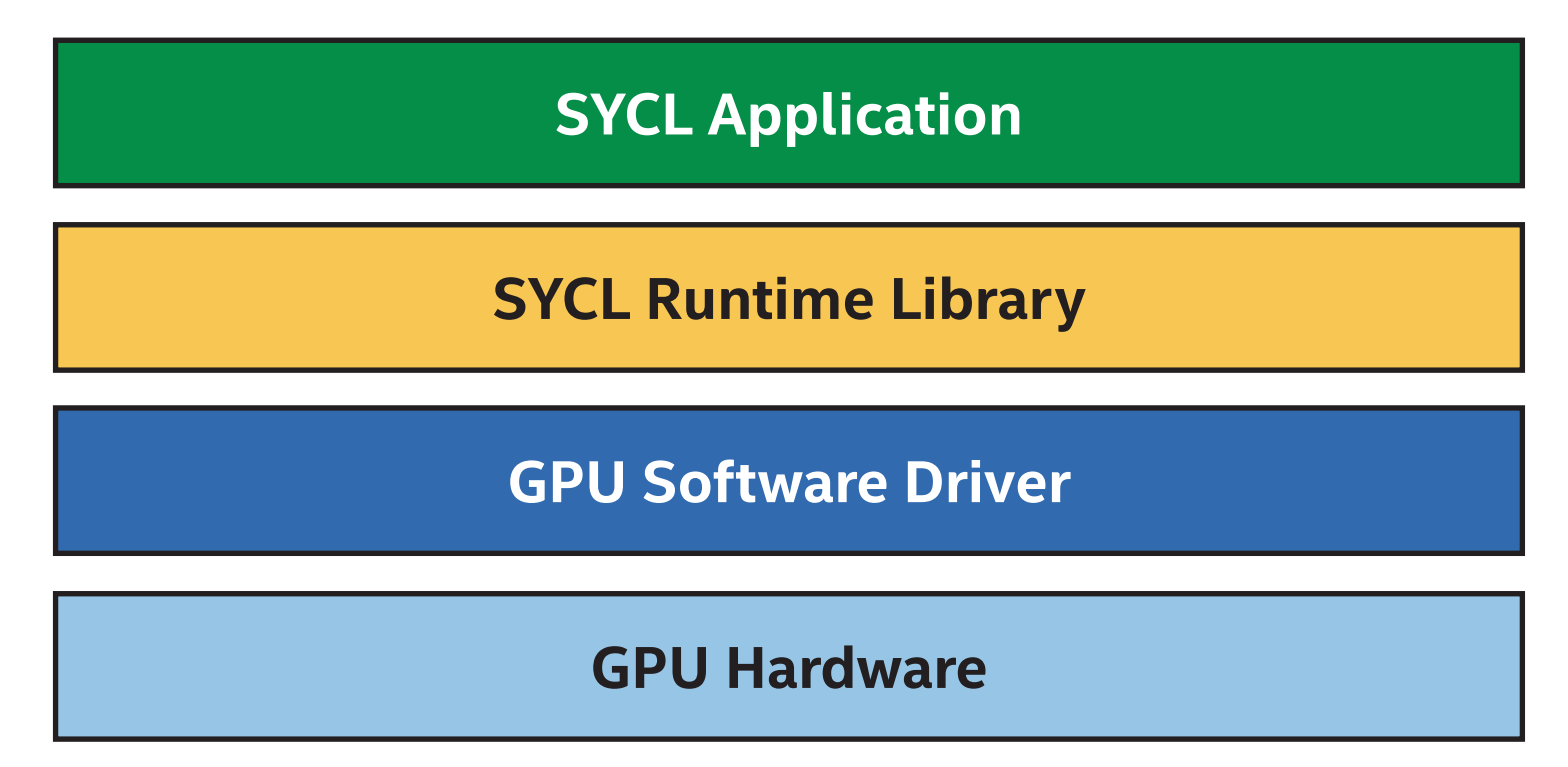
\includegraphics[width=1.0\textwidth]{content/chapter-15/images/10}
\end{center}

\hspace*{\fill} \par %插入空行
\textbf{SYCL运行时库}

SYCL运行库是SYCL应用程序交互的主要软件库。运行时库负责实现类,如队列、缓冲区和访问器,以及这些类的成员函数。运行时库的部分实现可能位于头文件中,因此可以直接编译为应用程序可执行文件。运行时库的其他部分作为库函数实现,这些库函数作为应用程序构建过程的一部分链接到应用程序可执行文件。运行时库通常不是特定于设备的,同一个运行时库可能会将负载分配到CPU、GPU、FPGA或其他设备上。\par

\hspace*{\fill} \par %插入空行
\textbf{GPU软件驱动}

虽然从理论上讲,SYCL运行库可以直接加载给GPU,但在实践中,大多数SYCL运行库都与GPU软件驱动程序接口,以便将工作提交给GPU。\par

GPU软件驱动程序通常是API的实现,如OpenCL、Level Zero或CUDA。大多数GPU软件驱动程序是在SYCL运行时调用的用户模式驱动程序库中实现的,用户模式驱动程序可以调用操作系统或内核模式驱动程序来执行系统级的任务,比如:分配内存或向设备提交工作。用户模式驱动程序也可以调用其他用户模式库,例如:GPU驱动程序可以调用GPU编译器来实时编译一个内核,从中间表示到GPU ISA(指令集架构)。各个软件模块,及其相互作用如图15-15所示。\par

\hspace*{\fill} \par %插入空行
图15-15 GPU软件驱动模块
\begin{center}
	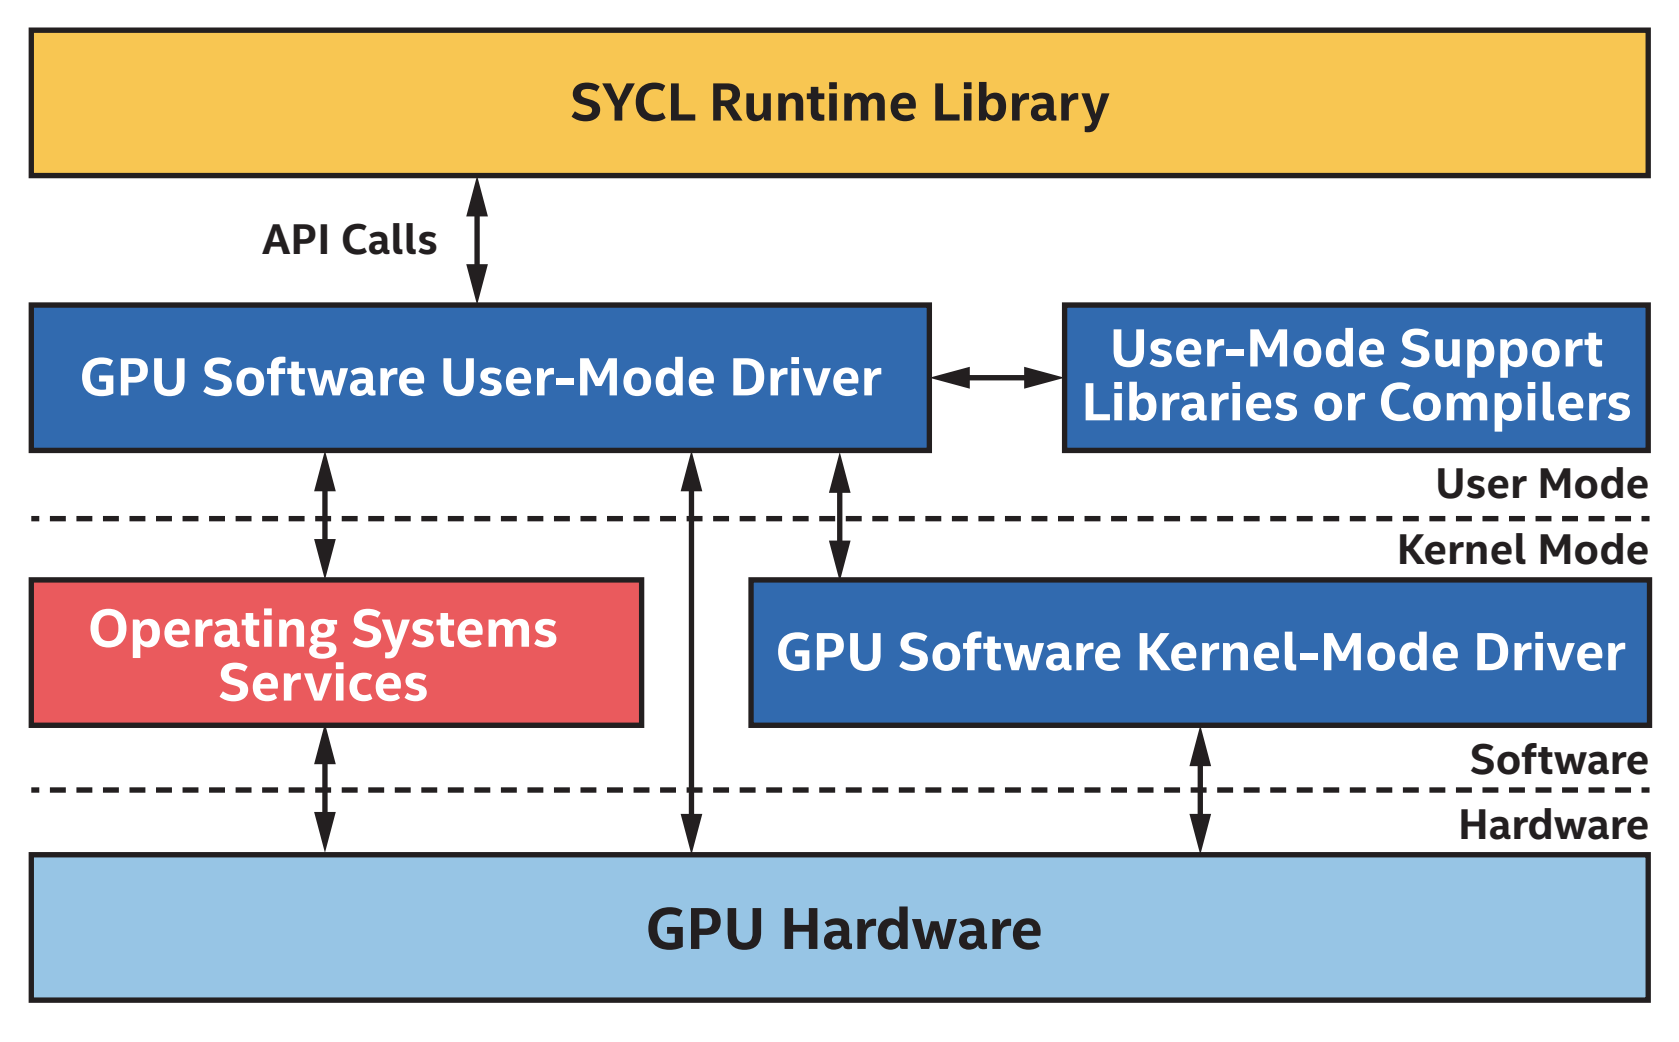
\includegraphics[width=1.0\textwidth]{content/chapter-15/images/11}
\end{center}

\hspace*{\fill} \par %插入空行
\textbf{GPU硬件}

当运行时库或GPU软件用户模式驱动程序被显式请求提交工作时,或者GPU软件启发式地决定应该开始工作时,通常会通过操作系统或内核模式驱动程序调用来开始在GPU上执行工作。某些情况下,GPU软件用户模式驱动程序可能会直接向GPU提交工作,但这并不常见,并且可能不是所有设备或操作系统都支持。\par

当工作在GPU上执行的结果需要在主机处理器或另一个加速器,GPU必须发出工作完成的信号。工作完成所涉及的步骤与工作提交的步骤非常相似,但执行方式是相反的:GPU可能会向操作系统或内核驱动程序发出信号,表示它已经完成了执行,然后用户模式驱动程序会得到通知,最后运行时库会通过GPU软件API调用观察到相应的工作已经完成。。\par

每一个步骤都引入了延迟,运行库和GPU软件需要在较低的延迟和较高吞吐量之间进行权衡。例如,频繁地向GPU提交工作可能会减少延迟,但频繁地提交也可能由于提交产生的开销而降低吞吐量。收集大量的工作将增加延迟,但将提交开销分摊到更多的工作上,并引入更多并行执行的机会。运行时和驱动都作出了正确的权衡,但如果怀疑驱动启发式的提交导致工作效率低下,应该咨询文档是否有方法来替代默认驱动程序行为,这里可能会使用特定于API,甚至是使用特定的机制。\par

\hspace*{\fill} \par %插入空行
\textbf{注意加载成本!}

尽管SYCL实现和GPU供应商正在不断创新和优化,以降低将工作转移到GPU的成本,但在启动GPU工作和在主机或其他设备上观察结果时,总是会有开销。当选择在哪里执行算法时,要考虑在设备上执行算法的好处,以及将算法和需要的数据移动到设备上的成本。某些情况下,最有效的方法可能是使用主机处理器执行并行操作——或者在GPU上低效地执行算法的串行部分——以避免将算法从一个处理器移动到另一个处理器的开销。\par

\begin{tcolorbox}[colback=red!5!white,colframe=red!75!black]
从整体上考虑算法的性能——在设备上执行算法的部分效率可能最高,而不是将执行转移到另一个设备上!
\end{tcolorbox}

\hspace*{\fill} \par %插入空行
\textbf{与设备存储器之间的传输}

对于使用专用内存的GPU,要特别注意内存和主机或其他设备上内存之间的传输成本。系统中不同内存类型的内存带宽差异如图15-16所示。\par

\hspace*{\fill} \par %插入空行
图15-16 设备内存、远程内存和主机内存之间的差异
\begin{center}
	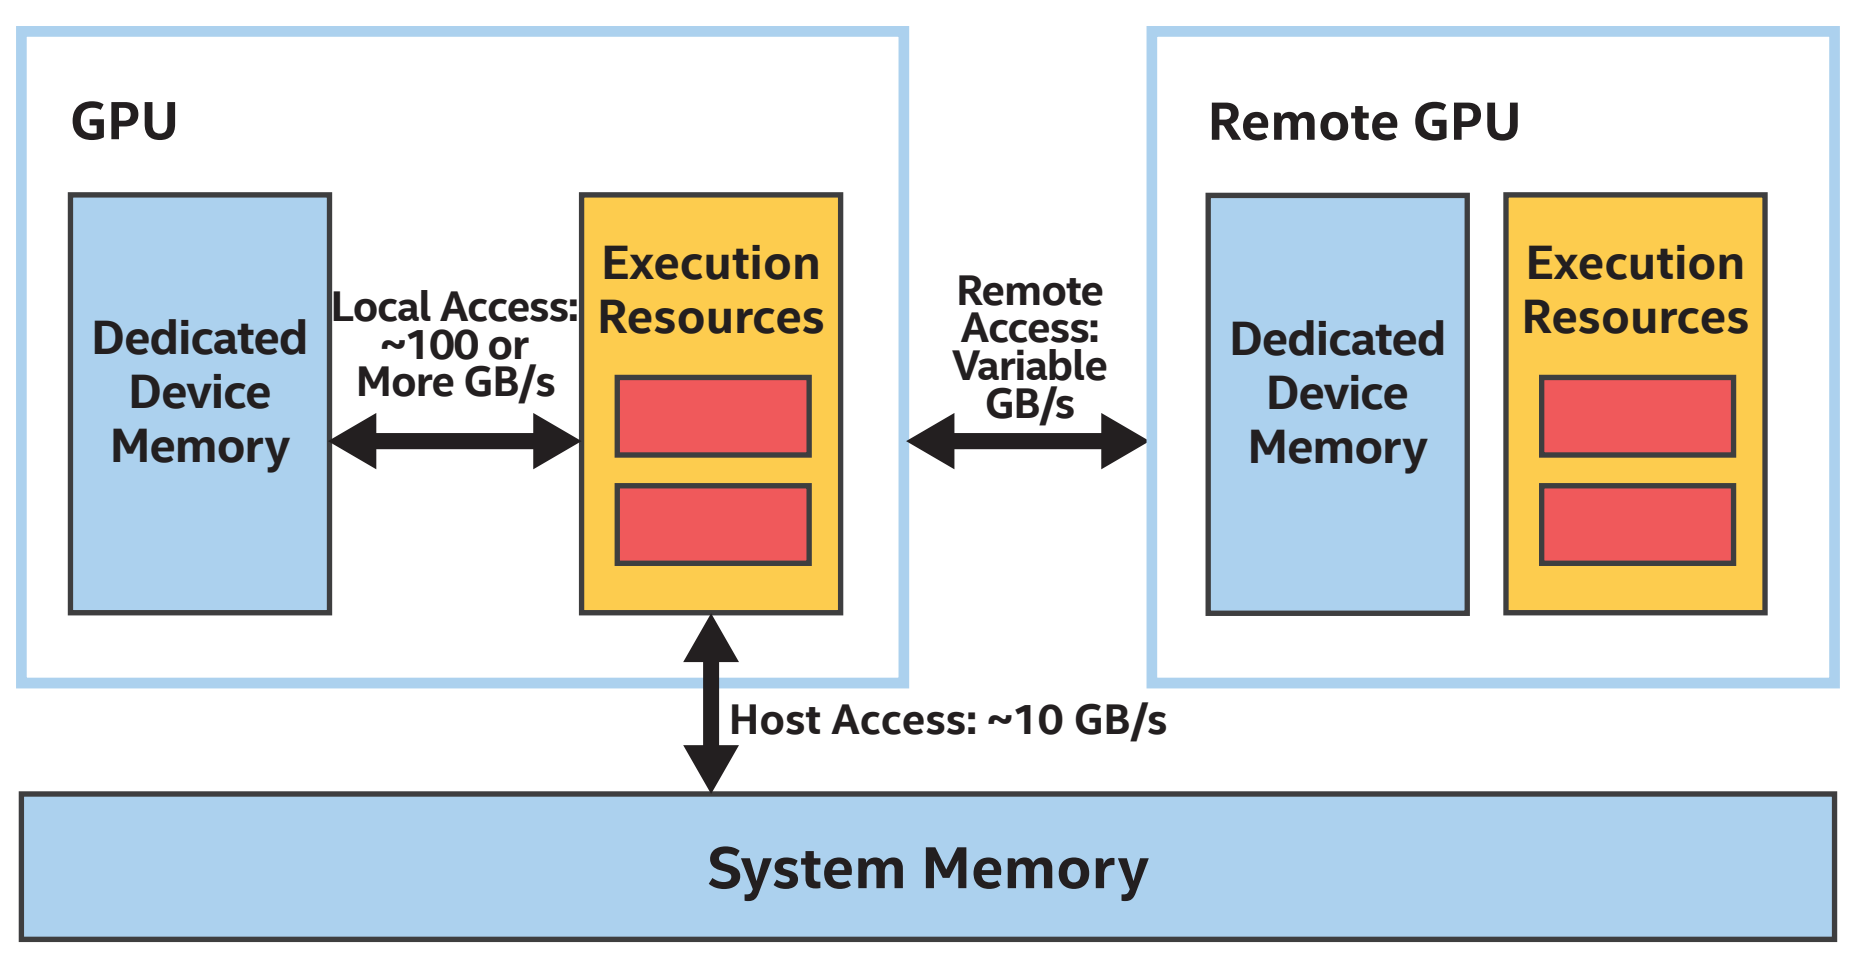
\includegraphics[width=1.0\textwidth]{content/chapter-15/images/12}
\end{center}

回顾一下第3章,GPU更喜欢在专用设备内存上运行,这比在主机内存或其他设备内存上运行要快多个数量级。尽管访问专用设备内存比访问远程内存或系统内存要快得多,但如果数据尚未在专用设备内存中,则必须复制或迁移数据。\par

频繁访问数据的话,将其移到专用设备内存中是性能有益的,特别是当GPU执行资源忙于处理另一个任务时,传输任务可以异步执行。当数据访问频率不高或不可预测时,最好是节省传输成本,并在远程或系统内存中操作数据(即使每次访问成本更高)。第6章描述了控制内存分配和复制和预取数据到专用设备内存的不同技术的方法。这些技术在为GPU优化程序执行时非常重要。\par








